\documentclass{standalone}

\usepackage{graphicx}
\usepackage{tabularx,multirow,colortbl,booktabs}

\usepackage{tikz}
\usetikzlibrary{calc}
\usetikzlibrary{positioning}
\tikzset{
    between/.style args={#1 and #2}{
    	at = ($(#1)!0.5!(#2)$)
    }
}

\begin{document}

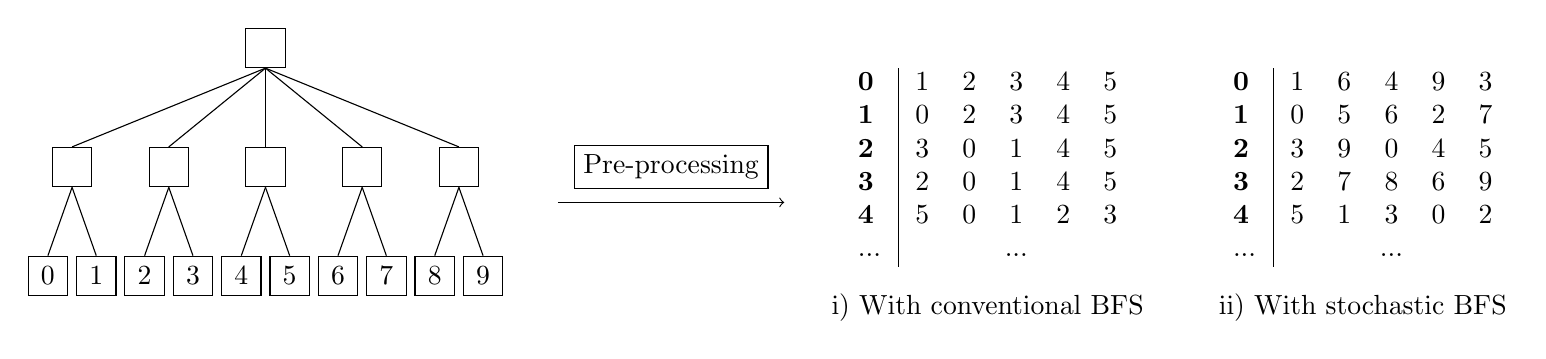
\begin{tikzpicture}[
        every node/.style={node distance=10mm and 1mm},
        server/.style={rectangle, draw=black, minimum size=.5cm},
        switch/.style={rectangle, draw=black, minimum size=.5cm},
    ]

    \node[server]      (S1)                       {0};
    \node[server]      (S2)        [right=of S1]  {1};
    \node[server]      (S3)        [right=of S2]  {2};
    \node[server]      (S4)        [right=of S3]  {3};
    \node[server]      (S5)        [right=of S4]  {4};
    \node[server]      (S6)        [right=of S5]  {5};
    \node[server]      (S7)        [right=of S6]  {6};
    \node[server]      (S8)        [right=of S7]  {7};
    \node[server]      (S9)        [right=of S8]  {8};
    \node[server]      (S10)       [right=of S9]  {9};

    \node[] 		 (H1) 		 [between=S1 and S2] {};
    \node[] 		 (H2) 		 [between=S3 and S4] {};
    \node[] 		 (H3) 		 [between=S5 and S6] {};
    \node[] 		 (H4) 		 [between=S7 and S8] {};
    \node[] 		 (H5) 		 [between=S9 and S10] {};

    \node[switch]      (E1)        [above = of H1] {};
    \node[switch]      (E2)        [above = of H2] {};
    \node[switch]      (E3)        [above = of H3] {};
    \node[switch]      (E4)        [above = of H4] {};
    \node[switch]      (E5)        [above = of H5] {};

    \node[switch]      (M1)        [above = of E3] {};

    \draw[-] (S1.north)  -- (E1.south);
    \draw[-] (S2.north)  -- (E1.south);
    \draw[-] (S3.north)  -- (E2.south);
    \draw[-] (S4.north)  -- (E2.south);
    \draw[-] (S5.north)  -- (E3.south);
    \draw[-] (S6.north)  -- (E3.south);
    \draw[-] (S7.north)  -- (E4.south);
    \draw[-] (S8.north)  -- (E4.south);
    \draw[-] (S9.north)  -- (E5.south);
    \draw[-] (S10.north)  -- (E5.south);

    \draw[-] (E1.north)  -- (M1.south);
    \draw[-] (E2.north)  -- (M1.south);
    \draw[-] (E3.north)  -- (M1.south);
    \draw[-] (E4.north)  -- (M1.south);
    \draw[-] (E5.north)  -- (M1.south);

    \node (PP) [shape = rectangle, draw, right=1.2cm of E5] {Pre-processing};

    \node (LH1) [left=.2cm of PP] {};
    \node (LH2) [right=.2cm of PP] {};
    \node (LH3) [below=.2cm of LH1] {};
    \node (LH4) [below=.2cm of LH2] {};

    \draw[->] (LH3) -- (LH4);

    \node (TD) [shape=rectangle, right=.8cm of PP] {
        \begin{tabular}{l | l l l l l }
            \textbf{0} & 1 & 2 & 3 & 4 & 5 \\
            \textbf{1} & 0 & 2 & 3 & 4 & 5 \\
            \textbf{2} & 3 & 0 & 1 & 4 & 5 \\
            \textbf{3} & 2 & 0 & 1 & 4 & 5 \\
            \textbf{4} & 5 & 0 & 1 & 2 & 3 \\
            ... & \multicolumn{5}{c}{...}\\
        \end{tabular}
    };

    \node (CD) [below=.1cm of TD] {i) With conventional BFS};

    \node (TR) [shape=rectangle, right=.8cm of TD] {
        \begin{tabular}{l | l l l l l }
            \textbf{0} & 1 & 6 & 4 & 9 & 3 \\
            \textbf{1} & 0 & 5 & 6 & 2 & 7 \\
            \textbf{2} & 3 & 9 & 0 & 4 & 5 \\
            \textbf{3} & 2 & 7 & 8 & 6 & 9 \\
            \textbf{4} & 5 & 1 & 3 & 0 & 2 \\
            ... & \multicolumn{5}{c}{...} \\
        \end{tabular}
    };

    \node (CR) [below=.1cm of TR] {ii) With stochastic BFS};

\end{tikzpicture}

\end{document}